% REV00 Tue 20 Jul 2021 08:12:01 WIB
% START Tue 20 Jul 2021 08:12:01 WIB

\chapter{Kelima}

% 11
\begin{figure}[htbp]
% h: here, where the figure appears in the text (use can always just use [h] )
% t: top,  top of the current page.
% b: bottom of the current page.
% p: page, top of the next available float space (sometimes end up being the end of the document).
\centerline{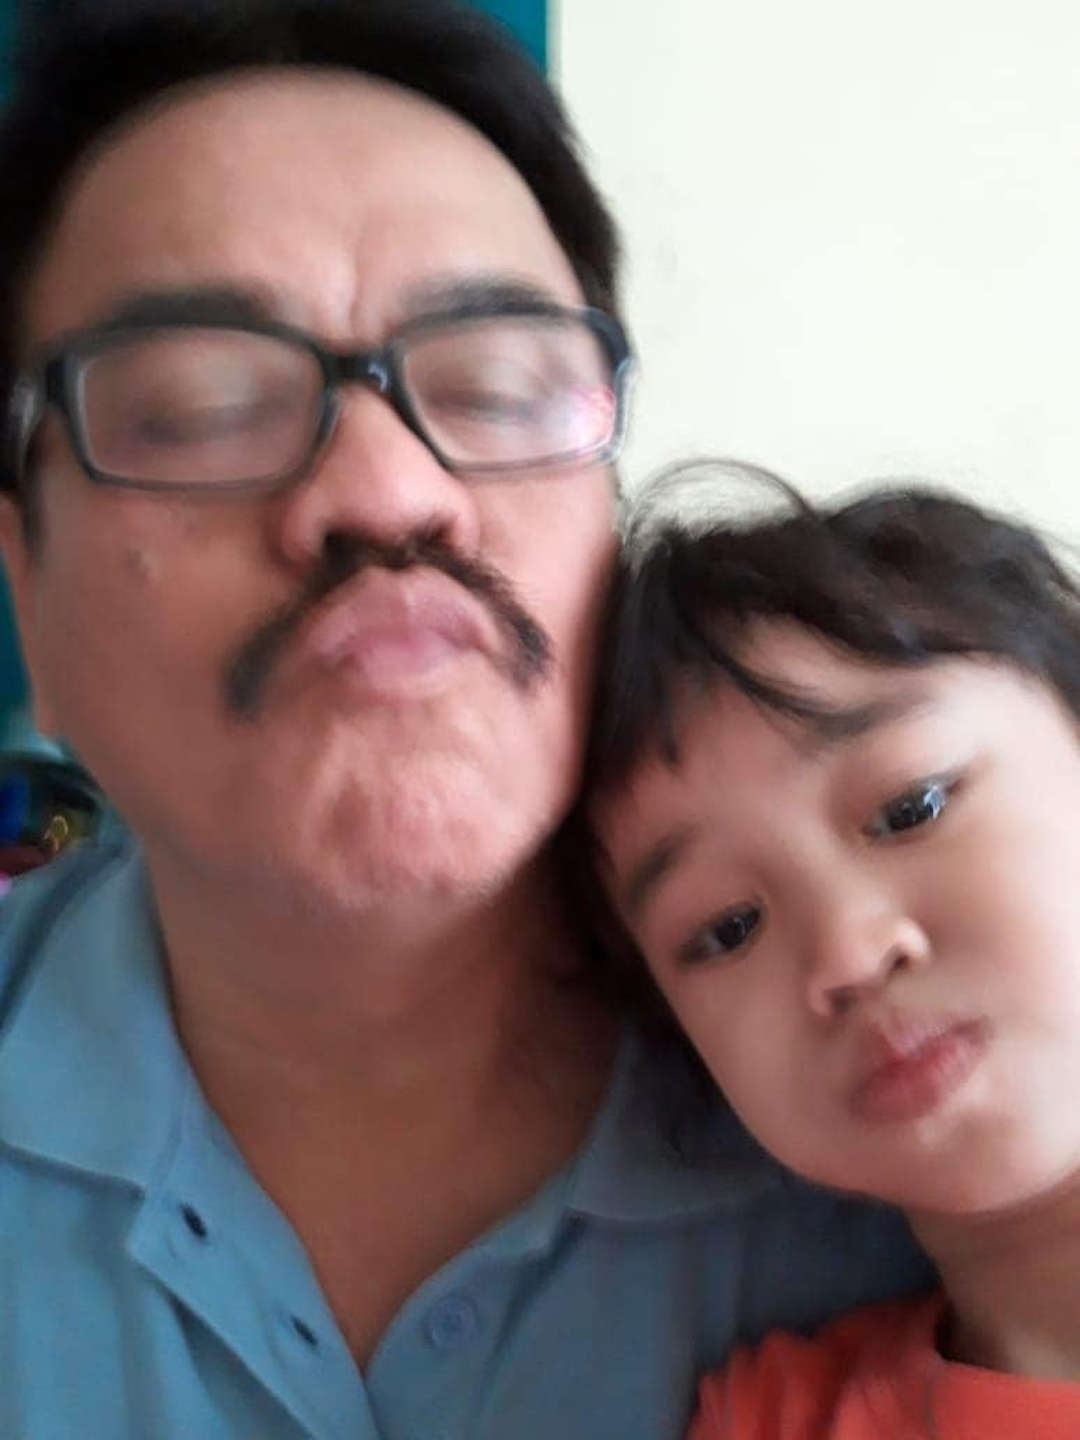
\includegraphics[scale=1.0]{01-05-01}}
\caption{“Satiri dan cucu: Keluarga adalah nomor satu”. Sumber: FB Satiri M Zen.}
\label{01-05-01}
\end{figure}
%

SATIRI adalah nama unik klasik Betawi. Saya belum pernah menemukan nama itu pada suku-suku atau bangsa-bangsa lain manapun di dunia. Keturunan Betawi masa kini juga tidak ada yang menggunakan nama itu. Anda tahu, klasik itu artinya membawa nilai-nilai abadi keindahan dan kebenaran. Seperti musik klasik, atau fisika klasik. Dan unik adalah perjalanan hidup sobatku yang satu ini, Satiri.

Pada Semester terakhir kelas III SMA, negara mulai menyelenggarakan proses penerimaan mahasiswa perguruan tinggi negeri (PTN). Dibuatlah skema Proyek Perintis-1 untuk ujian nasional masuk PTN kelas-1 seperti ITB, UI, UGM dan IPB; Perintis-2 untuk seleksi masuk PTN kelas-1 berdasarkan nilai Rapor, tanpa harus ujian; Perintis-3 untuk ujian nasional masuk PTN kelas-2; dan Perintis-4 untuk ujian nasional masuk IKIP, universitas pendidikan, alias calon guru sekolah.

Bagaimana dengan Satiri? Selepas semester-5 di SMA, dia termasuk elit yang boleh ikut mendaftar Perintis-2. Ini membuatnya tercenung cukup lama. Bagaimana dengan uang kuliahnya nanti? Bayar praktikumnya berapa? Yaah, daftar dulu sajalah, urusan belakangan, mumpung boleh daftar dan gratis. Semoga Tuhan nanti kasih jalan.

Sejauh mampu dia pikir, maka masuk FMIPA UI Jakarta adalah satu-satunya pilihan. Oia, harus diingat juga bahwa Perintis-2 itu dibatasi untuk masuk ke universitas pada jurusan matematika dan sains saja. Belakangan kita tahu bahwa sebenarnya kebijakan pemerintah Indonesia saat itu sangatlah tepat: Kalau Indonesia mau maju, sains harus menjadi basis yang kuat untuk pengembangan teknologi, harus diisi oleh orang-orang pintar, juara-juara di SMA.

Satiri hanya bisa berpikir, bahwa untuk menyambung kuliahnya nanti di Kampus Salemba, dia bisa naik sepeda dan tetap dagang kembang. Ya, hanya itu yang dia tahu.

Pengumuman Perintis-2 datang di sekitar pengumuman kelulusan SMA. Ujian Perintis-1 baru dilakukan sekitar 2 bulan setelah kita terima ijazah. DI SMA XI Bulungan, diumumkanlah bahwa Satiri diterima di FMIPA ITB, bukan di UI seperti yang ia lamar. Loh, koq bisa begitu? (OMG, how comes?)

Bertanyalah Satiri kepada salah seorang guru, Pak Meilani. Saya kebetulan kenal guru tersebut, karena beliau nyambi sebagai guru di SMA saya: SMA swasta tak ‘berkelas’.

“Pak, ini mengapa saya melamar ke UI diterima di ITB?”

“Ah, elo Tong, dasar anak Betawi. Sudah bagus diterima di ITB. Kalau nggak, anak Betawi kan paling juga jadi pedagang buah”, katanya rada ketus. Menggunakan logat Betawi pula dia…

“Yaah, Bapak…”

Berhari-hari dia berpikir keras, bagaimana dia bisa ke ITB? Seumur hidup dia belum pernah keluar dari tanah Betawi! Bagaimana dengan uang kos? Buntu pikirannya. Duh, Tuhan…

Dan Tuhan pun mendengar keluhannya, memberanikan kakinya untuk merangkak lagi menghadap Pak Lesilolo, sang legenda, Kepala Sekolah yang diyakini menjadikan SMAN XI sebagai sekolah terbaik nasional.

“Bapak, ini mengapa saya melamar ke UI diterima di ITB? dan saya juga tidak tahu bagaimana akan ke ITB?”

“Kasih saya waktu beberapa hari yah…”, jawabnya singkat dengan tenang kebapakan. Agaknya dia punya jawaban dari semua pertanyaan.

Tunggu. Something should be very wrong. Karena pertanyaan pertama Satiri itu tidak dijawab, maka dia jadi tahu bahwa SMAN XI memang sengaja menjebloskan Satiri ke ITB, sekolah MIPA yang dianggap terbaik nasional saat itu.

Sesuai janji, lepas beberapa hari Satiri dipanggil untuk menghadap Kepala Sekolah. Satiri sudah ambil ancang-ancang untuk membalas perbuatan kepala sekolah yang menjebloskannya ke ITB. “Awas kamu…”

Tanpa pendahuluan apapun, kepala sekolah langsung mengatakan: “Kamu nanti tanggal sekian jam 7 malam datang ke sini yah…”, seraya memberikan secarik kertas. Di situ tertulis nama Jenderal “O” dan alamatnya di Kebayoran Baru. Belakangan Satiri tahu bahwa Jenderal O adalah Direktur Utama salah satu BUMN. Di jaman orde baru ya semua memang serba militer. Satiri lupa akan niat pembalasannya.

Kata orang-orang pintar, lupa itu bagian dari nikmat dan keselamatan dari Tuhan.

Dikipas-kipasilah dirinya untuk datang ke rumah sang Jenderal pada Hari-H dan Jam-J yang sudah ditentukan Sang Legenda. Dalam hatinya, pokoknya kalau disuruh apapun aku harus bilang “mau”, asalkan bisa kuliah di Bandung. Tidak ditempeleng sang Jenderal juga sudah bagus kan..

“Selamat malam Pak Jenderal…”, sapanya sambil mencium tangan sang Jenderal. Mencium tangan ibundanya berpamitan tadi, itulah yang nomor satu, kebiasaan dia.

“Malam. Katanya kamu anak pintar yah?”, langsung boss menyergap, khas Jenderal.

“Eh, anu Pak, eeh…”

“Kamu mau minta beasiswa dari saya?”

“Eh, anu Pak, saya, eeh… Mau Pak, mau…”

“Kamu mau kalau sambil kuliah saya tugaskan juga bekerja di perusahaan Cabang Bandung?”

“Mau Pak, mau…”, jawab Satiri lebih mantap dari sebelumnya. Ada angin segar lewat.

“Kamu mau hanya dikasih uang seadanya untuk kuliah?”

“Mau Pak, mau…”

“Kamu mau saya kasih kamar kontrakan kecil di Gang kecil yang becek?”

“Mau Pak, mau…”

“Mau kamu saya suruh jadi salesman produk kami, berdagang keliling kampung di sekitaran Bandung?

“Mau Pak, mau…”

“Kamu ini ya… Koq mau-mau terus? Kamu itu sebenarnya mau kuliah, atau mau kerja?” hardik sang Jenderal.

“Kuliah saya mau. Kerja juga saya mau Pak”. Mantap.

Untuk beberapa saat, tercenung juga sang Jenderal mengamati Satiri. Mungkin dia sedang melihat dirinya waktu seumuran Satiri. Belakangan Satiri mengatakan kepadaku bahwa Jenderal O tidak dikaruniai anak kandung, tetapi punya satu anak angkat yang baik hati. Akhirnya,

“Baiklah, minggu depan akan saya sampikan keputusan kami kepada gurumu. Banyak berdoa saja yaah…”, tutup sang Jenderal. Dengan nada datar. Tidak ada kejelasan. O-ow…

Satiri hanya bisa terpukau lemas. Dan dia tetap harus mengatakan dengan tegar dan pasang senyum: “Terima kasih banyak Bapak Jenderal…”, seraya mencium tangan sang Jenderal.

Keluar dari rumah besar itu pandangannya kosong, penuh keraguan. Dia bahkan harus duduk di kedai rokok, menenangkan dirinya selama hampir setengah jam, sebelum mencari bus Blok M – Tanah Abang.

“Apa aku juga harus berdagang rokok seperti ini juga ya…”
\\[10pt]

Sumber tulisan asli \url{https://www.facebook.com/reno.alamsyah.94/posts/10226530419032813}

